\documentclass[12pt,fleqn]{article}\usepackage{../../common}
\begin{document}
Sonlu Öğeler - 2. Bölüm

Üzerinden geçelim, sistem zayıf form ile ise başlar. Önceki dersin sonunda
Galerkin fikrini tanıştırdık, sürekli diferansiyel denklem yerine onu ayrıksal
temsil etmeye uğraş. Galerkin bunun için bazı deneme fonsiyonları kullanır
onlara $\phi_1,...,\phi_N$ diyelim, ayrıca test fonksiyonları da vardır
(çoğunlukla test fonksiyonları ile deneme, yani $\phi$ ve $v$ fonksiyonları
aynıdır). Bugün işleyeceğimiz bu fonksiyonların nasıl seçildiği ve hazirlik
asamasini gosterdikten sonra bunun verdigi $KU = F$ denklemin nasil
cozuldugu. $K$ nereden geliyor, $F$ nereden geliyor? $F$ bir sekilde alttaki
ikinci denklemin (oktan sonra) sag tarafindan geliyor, $K$ ise sol
tarafindan.. Detaylari simdi gorecegiz.

$$
- \frac{\ud}{\ud x} \left( c(x) \frac{\ud u}{\ud x} \right) = f(x) \to
\int _{0}^{1} c \frac{\ud u}{\ud x} \frac{\ud v}{\ud x} \ud x =
\int _{0}^{1} f(x) v(x) \ud x
$$

ki eger $u(1)=0$ ise $v(1) = 0$ (sinir sarti).

Sonlu ogelerin temeli $KU = F$. Ustteki denklemde okun sol tarafi diferansiyel
denklemimiz, sinir sartlari vs ile ``guclu formda'', oktan sonrasi zayif form,
ki onun da kendi sinir sartlari var. Sabit degiskenler guclu formdan zayif forma
geciyor, ama serbest degiskenler gecmiyor. $v$'yi $u$'dan olan ufak sapmalar
olarak gordugum icin eger $u$'yi sabitliyorsam $v$ de sabitleniyor.

Tum bunlari gorduk ama hala ayaklarimiz yere basmadi; bir cok fikirden
bahsettik, ama simdi daha gercek dunyaya baglanacagiz. Gercek dunya demek tabii
$\phi$'lerle alakali, hangi somut fonksiyonlari $\phi$ olarak sececegiz?

Acaba ornek bir $\phi$ ne olabilir? Mesela $x=2$ noktasinda tepe yapan bir
parcali lineer fonksiyon kullanabilirim,

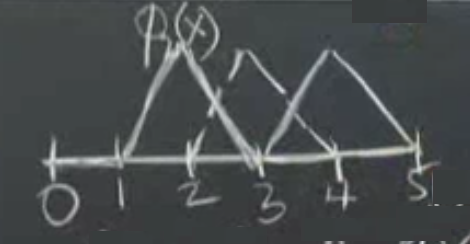
\includegraphics[width=10em]{compscieng_1_18_01.png}

Bu fonksiyona $\phi_2(x)$ diyelim, 1 ila 3 arasinda 2 uzerinde tepe yapiyor
diger yerlerde ya lineer egimi var, ya da degeri sifir. Onun sagindaki $\phi_3$
olabilir, benzer bir fonksiyon sadece 3 degeri bazli tanimli. Buradaki
ana amac sistemi basit ogeler uzerinde insa etmek. Sonlu ogelerin ana fikri
budur; $\phi$ icin basit fonksiyonlar kullan. Bu basitligin devami olarak
$\phi$ ve $v$ fonksiyonlarini ayni sec.

Peki sinir noktalarinda ne olacak? 


















[devam edecek]

\end{document}

















